%#!pdfpLaTeX
%
% 北村研究室用特論予稿のTeXテンプレートファイル
% 本ファイルは非公式であり,下記で公開されているワードのテンプレートが公式である.
% https://www.kagawa-nct.ac.jp/EE/local/index.html (学内限定アクセス)
%
% 2020年1月18日 北村大地作成
%

\documentclass[a4j,10pt]{jsarticle}
\usepackage{nitkagawaprocas} % 予稿テンプレートクラスファイル
\usepackage{amsmath,amssymb} % 数式環境
\usepackage{bm} % 数式の太字斜体
\usepackage[dvipdfmx]{color}
\usepackage[dvipdfmx]{graphicx}
\usepackage{flushend} % 2段組みの最終ページの高さを揃える

\renewcommand{\baselinestretch}{0.8} % 行間設定(標準は0.8)

%%%%%%%%%%%%%%%%%%%%%%%%%%% 論文情報 %%%%%%%%%%%%%%%%%%%%%%%%%%%

%%%%% タイトル %%%%%
\title{特別研究I・II発表審査会 特別研究論文概要\\の作成要領}

%%%%% 著者 %%%%%
\author{高専 太郎}
\eauthor{Kosen Tarou}

%%%%% 所属 %%%%%
\affiliation{創造工学専攻}

%----- 図表題が英語の場合は次の2行を有効化 -----%
%\renewcommand{\figurename}{Fig.~} 
%\renewcommand{\tablename}{Table~}
%--------------------------------------------%

\begin{document}
\maketitle% タイトル生成

%----- ハイフン付きページ番号を表示する場合は次3行を有効化 -----%
\setcounter{page}{1} % 開始ページ番号(3にすると3ページと4ページの2枚になる)
\pagestyle{hyphenpage}
\thispagestyle{hyphenpage}
%---------------------------------------------------------%

%----- ハイフン無しページ番号を表示する場合は次3行を有効化 -----%
%\setcounter{page}{1} % 開始ページ番号(3にすると3ページと4ページの2枚になる)
%\thispagestyle{plain}
%\pagestyle{plain}
%---------------------------------------------------------%

%----- ページ番号を削除する場合は次3行を有効化 -----%
%\thispagestyle{empty}
%\pagestyle{empty}
%-----------------------------------------------%

%%%%%%%%%%%%%%%%%%%%%%%%%%% 本文 %%%%%%%%%%%%%%%%%%%%%%%%%%%
%----------------------------------------------
\section{ページ設定とページ数}
%----------------------------------------------

マージンは左右が20mm,上方が20mm,下方が25mm程度とし,
2段組で1段25文字50行を標準とします.
段幅は約82mmです.用紙はA4を縦置きで使用.
ページ総数は2ページとし,過不足は認めません.

%----------------------------------------------
\section{タイトルページ}
%----------------------------------------------

タイトルページは2つの部分で構成されます.
\begin{itemize}
\item タイトル部分(題目,所属,著者は上記のように並べて下さい)
\item 本文部分:横2段組
\end{itemize}

%----------------------------------------------
\subsection{タイトル部分のレイアウトとフォント}
%----------------------------------------------

タイトル部分の左右のマージンは、本文の左右のマージンよりも
それぞれ1~cmずつ大きくとって下さい.
したがって,A4用紙の幅に対して左右それぞれ3~cmずつのマージンを
とります.

タイトルはA4用紙の上辺に約 3 cm のマージンを取り,
センタリングします.
以下次の順にタイトル部分の構成要素を書いて下さい.

和文タイトル:ゴチック体 20 pt フォント

和文所属著者名:明朝体 12 pt フォント

%----------------------------------------------
\subsection{本文部分のレイアウトとフォント}
%----------------------------------------------

本文は2段組で,左右のマージンは20~mm ずつ,段と段との
間のスペースは約6~mm とします.下辺のマージンは25~mmです.

本文には明朝体10~ptフォントを用いて下さい.

%----------------------------------------------
\section{一般ページ}
%----------------------------------------------

第2ページ以降の通常のページは上辺のマージンを20~mmとします.
それ以外はタイトルページの本文部分と同じレイアウトとフォントで
本文を作成します.

%----------------------------------------------
\section{数式および数学記号}
%----------------------------------------------
数式や数学記号は次の式(\ref{eq:G})
\begin{align}
  G = \sum_{n=0}^{\infty} b_n(t) \label{eq:G}
\end{align}
のように本文と独立している場合でも,$C_D$,$\alpha(z)$の
ように文章の中に出てくる場合でも同じ数式用のフォントを用いて
作成します.

数式はセンタリングし,式番号は括弧書きで右詰めにします.

%----------------------------------------------
\section{図表}
%----------------------------------------------

図表はそれらを最初に引用する文章と同じページに置くことを
原則とします.原稿末尾にまとめたりしてはいけません.

図表を引用する場合は図\ref{fig:sample}および
表\ref{table:sample}のように記述して下さい.

%-%-%-%-%-%-%-%-%
\begin{table}[t]
  \centering
  \caption{表のキャプションは表の上の中央に置く.このように長いときはインデントして折り返す}
  \label{table:sample}
  \vspace{0pt} % キャプション下部の余白調整
  \begin{tabular}{|c|c|c|} \hline
    実験番号 & 水深 [m] & 流量 [$\mathrm{m}^3/\mathrm{s}$] \\ \hline
    1 & 2.5 & 10.0 \\ \hline
    2 & 3.8 & 20.0 \\ \hline
    3 & 4.5 & 30.0 \\ \hline
  \end{tabular}
  \vspace{10pt} % 表下部の余白調整
\end{table}
%-%-%-%-%-%-%-%-%

%-%-%-%-%-%-%-%-%
\begin{figure}[t]
  \centering
  \vspace{0pt} % 図上部の余白調整
  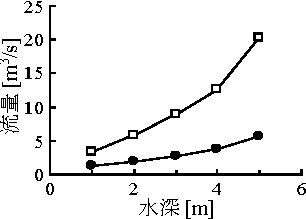
\includegraphics[width=0.75\columnwidth]{graph.pdf}
  \vspace{0pt} % 図とキャプション間の余白調整
  \caption{図のキャプションは図の下の中央に置く.}
  \vspace{0pt} % キャプション下部の余白調整
  \label{fig:sample}
\end{figure}
%-%-%-%-%-%-%-%-%

%----------------------------------------------
\section{参考文献}
%----------------------------------------------

参考文献は\cite{sample1}と表記して引用してください.
複数の文献を引用する場合は\cite{sample1,sample2,sample3}または
\cite{sample1}--\cite{sample3}と記述してください.

%----------------------------------------------
\section{注意事項}
%----------------------------------------------

本テンプレートは元々Wordでのみ配布されている予稿の
テンプレートを北村大地がLaTeXによる組版で可能な限り忠実に
再現したファイルになります.マージンや余白などには細心の
注意を払いましたが,ボールドフォントの違い等の細かい点は
組版ソフトの違いが存在する以上生じてしまいます.
あくまでも非公式のテンプレートとして自己責任で使用してください.

TeXのコンパイラは恐らく最もスタンダードであるpdfpLaTeXを使用
することを想定しています.他のコンパイラでの動作確認はして
おりません.また,今後の対応の予定もありません.もう北村は
疲れました.


%%%%% 参考文献 %%%%%
\begin{thebibliography}{9}% 10以上の文献数であれば99とする

\bibitem{sample1}
  T.~Kosen and H. Takamatu,
  ``First paper title goes here,''
  {\it Journal Name}, vol.~1, no.~1, pp.~1--10, 2018.

\bibitem{sample2}
  T.~Kosen, H. Takamatu, and S. Takuma, 
  ``Second paper title goes here,''
  {\it Journal Name}, vol.~2, no.~2, pp.~11--20, 2019.

\bibitem{sample3}
  T.~Kosen and H. Takamatu,
  ``Third paper title goes here,''
  {\it Journal Name}, vol.~3, no.~3, pp.~21--30, 2020.

\end{thebibliography}

\end{document}